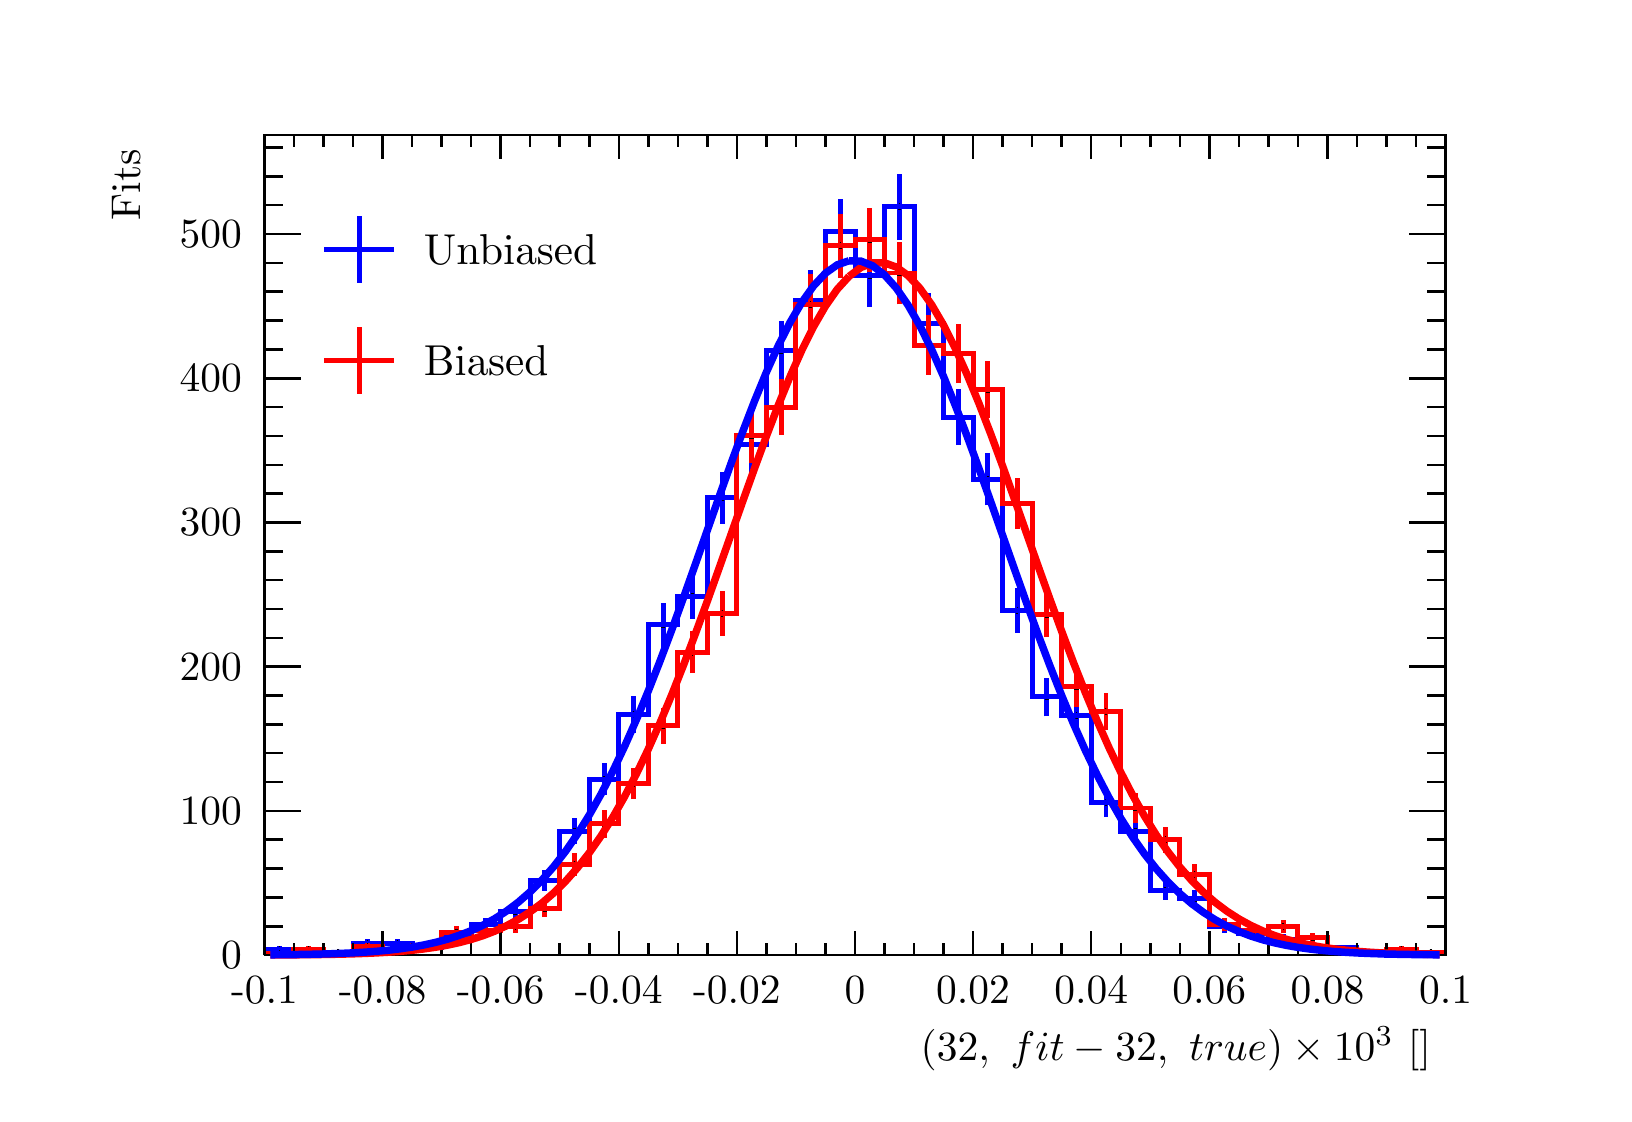
\begin{tikzpicture}
\pgfdeclareplotmark{cross} {
\pgfpathmoveto{\pgfpoint{-0.3\pgfplotmarksize}{\pgfplotmarksize}}
\pgfpathlineto{\pgfpoint{+0.3\pgfplotmarksize}{\pgfplotmarksize}}
\pgfpathlineto{\pgfpoint{+0.3\pgfplotmarksize}{0.3\pgfplotmarksize}}
\pgfpathlineto{\pgfpoint{+1\pgfplotmarksize}{0.3\pgfplotmarksize}}
\pgfpathlineto{\pgfpoint{+1\pgfplotmarksize}{-0.3\pgfplotmarksize}}
\pgfpathlineto{\pgfpoint{+0.3\pgfplotmarksize}{-0.3\pgfplotmarksize}}
\pgfpathlineto{\pgfpoint{+0.3\pgfplotmarksize}{-1.\pgfplotmarksize}}
\pgfpathlineto{\pgfpoint{-0.3\pgfplotmarksize}{-1.\pgfplotmarksize}}
\pgfpathlineto{\pgfpoint{-0.3\pgfplotmarksize}{-0.3\pgfplotmarksize}}
\pgfpathlineto{\pgfpoint{-1.\pgfplotmarksize}{-0.3\pgfplotmarksize}}
\pgfpathlineto{\pgfpoint{-1.\pgfplotmarksize}{0.3\pgfplotmarksize}}
\pgfpathlineto{\pgfpoint{-0.3\pgfplotmarksize}{0.3\pgfplotmarksize}}
\pgfpathclose
\pgfusepathqstroke
}
\pgfdeclareplotmark{cross*} {
\pgfpathmoveto{\pgfpoint{-0.3\pgfplotmarksize}{\pgfplotmarksize}}
\pgfpathlineto{\pgfpoint{+0.3\pgfplotmarksize}{\pgfplotmarksize}}
\pgfpathlineto{\pgfpoint{+0.3\pgfplotmarksize}{0.3\pgfplotmarksize}}
\pgfpathlineto{\pgfpoint{+1\pgfplotmarksize}{0.3\pgfplotmarksize}}
\pgfpathlineto{\pgfpoint{+1\pgfplotmarksize}{-0.3\pgfplotmarksize}}
\pgfpathlineto{\pgfpoint{+0.3\pgfplotmarksize}{-0.3\pgfplotmarksize}}
\pgfpathlineto{\pgfpoint{+0.3\pgfplotmarksize}{-1.\pgfplotmarksize}}
\pgfpathlineto{\pgfpoint{-0.3\pgfplotmarksize}{-1.\pgfplotmarksize}}
\pgfpathlineto{\pgfpoint{-0.3\pgfplotmarksize}{-0.3\pgfplotmarksize}}
\pgfpathlineto{\pgfpoint{-1.\pgfplotmarksize}{-0.3\pgfplotmarksize}}
\pgfpathlineto{\pgfpoint{-1.\pgfplotmarksize}{0.3\pgfplotmarksize}}
\pgfpathlineto{\pgfpoint{-0.3\pgfplotmarksize}{0.3\pgfplotmarksize}}
\pgfpathclose
\pgfusepathqfillstroke
}
\pgfdeclareplotmark{newstar} {
\pgfpathmoveto{\pgfqpoint{0pt}{\pgfplotmarksize}}
\pgfpathlineto{\pgfqpointpolar{44}{0.5\pgfplotmarksize}}
\pgfpathlineto{\pgfqpointpolar{18}{\pgfplotmarksize}}
\pgfpathlineto{\pgfqpointpolar{-20}{0.5\pgfplotmarksize}}
\pgfpathlineto{\pgfqpointpolar{-54}{\pgfplotmarksize}}
\pgfpathlineto{\pgfqpointpolar{-90}{0.5\pgfplotmarksize}}
\pgfpathlineto{\pgfqpointpolar{234}{\pgfplotmarksize}}
\pgfpathlineto{\pgfqpointpolar{198}{0.5\pgfplotmarksize}}
\pgfpathlineto{\pgfqpointpolar{162}{\pgfplotmarksize}}
\pgfpathlineto{\pgfqpointpolar{134}{0.5\pgfplotmarksize}}
\pgfpathclose
\pgfusepathqstroke
}
\pgfdeclareplotmark{newstar*} {
\pgfpathmoveto{\pgfqpoint{0pt}{\pgfplotmarksize}}
\pgfpathlineto{\pgfqpointpolar{44}{0.5\pgfplotmarksize}}
\pgfpathlineto{\pgfqpointpolar{18}{\pgfplotmarksize}}
\pgfpathlineto{\pgfqpointpolar{-20}{0.5\pgfplotmarksize}}
\pgfpathlineto{\pgfqpointpolar{-54}{\pgfplotmarksize}}
\pgfpathlineto{\pgfqpointpolar{-90}{0.5\pgfplotmarksize}}
\pgfpathlineto{\pgfqpointpolar{234}{\pgfplotmarksize}}
\pgfpathlineto{\pgfqpointpolar{198}{0.5\pgfplotmarksize}}
\pgfpathlineto{\pgfqpointpolar{162}{\pgfplotmarksize}}
\pgfpathlineto{\pgfqpointpolar{134}{0.5\pgfplotmarksize}}
\pgfpathclose
\pgfusepathqfillstroke
}
\definecolor{c}{rgb}{1,1,1};
\draw [color=c, fill=c] (0,0) rectangle (20,13.5302);
\draw [color=c, fill=c] (3,1.75893) rectangle (18,12.1772);
\definecolor{c}{rgb}{0,0,0};
\draw [c,line width=0.9] (3,1.75893) -- (3,12.1772) -- (18,12.1772) -- (18,1.75893) -- (3,1.75893);
\definecolor{c}{rgb}{1,1,1};
\draw [color=c, fill=c] (3,1.75893) rectangle (18,12.1772);
\definecolor{c}{rgb}{0,0,0};
\draw [c,line width=0.9] (3,1.75893) -- (3,12.1772) -- (18,12.1772) -- (18,1.75893) -- (3,1.75893);
\draw [c,line width=0.9] (3,1.75893) -- (3.375,1.75893) -- (3.375,1.75893) -- (3.75,1.75893) -- (3.75,1.75893) -- (4.125,1.75893) -- (4.125,1.75893) -- (4.5,1.75893) -- (4.5,1.75893) -- (4.875,1.75893) -- (4.875,1.75893) -- (5.25,1.75893) --
 (5.25,1.75893) -- (5.625,1.75893) -- (5.625,1.75893) -- (6,1.75893) -- (6,1.75893) -- (6.375,1.75893) -- (6.375,1.75893) -- (6.75,1.75893) -- (6.75,1.75893) -- (7.125,1.75893) -- (7.125,1.75893) -- (7.5,1.75893) -- (7.5,1.75893) -- (7.875,1.75893)
 -- (7.875,1.75893) -- (8.25,1.75893) -- (8.25,1.75893) -- (8.625,1.75893) -- (8.625,1.75893) -- (9,1.75893) -- (9,1.75893) -- (9.375,1.75893) -- (9.375,1.75893) -- (9.75,1.75893) -- (9.75,1.75893) -- (10.125,1.75893) -- (10.125,1.75893) --
 (10.5,1.75893) -- (10.5,1.75893) -- (10.875,1.75893) -- (10.875,1.75893) -- (11.25,1.75893) -- (11.25,1.75893) -- (11.625,1.75893) -- (11.625,1.75893) -- (12,1.75893) -- (12,1.75893) -- (12.375,1.75893) -- (12.375,1.75893) -- (12.75,1.75893) --
 (12.75,1.75893) -- (13.125,1.75893) -- (13.125,1.75893) -- (13.5,1.75893) -- (13.5,1.75893) -- (13.875,1.75893) -- (13.875,1.75893) -- (14.25,1.75893) -- (14.25,1.75893) -- (14.625,1.75893) -- (14.625,1.75893) -- (15,1.75893) -- (15,1.75893) --
 (15.375,1.75893) -- (15.375,1.75893) -- (15.75,1.75893) -- (15.75,1.75893) -- (16.125,1.75893) -- (16.125,1.75893) -- (16.5,1.75893) -- (16.5,1.75893) -- (16.875,1.75893) -- (16.875,1.75893) -- (17.25,1.75893) -- (17.25,1.75893) -- (17.625,1.75893)
 -- (17.625,1.75893) -- (18,1.75893);
\draw [c,line width=0.9] (3,1.75893) -- (18,1.75893);
\draw [c,line width=0.9] (3,2.06336) -- (3,1.75893);
\draw [c,line width=0.9] (3.375,1.91115) -- (3.375,1.75893);
\draw [c,line width=0.9] (3.75,1.91115) -- (3.75,1.75893);
\draw [c,line width=0.9] (4.125,1.91115) -- (4.125,1.75893);
\draw [c,line width=0.9] (4.5,2.06336) -- (4.5,1.75893);
\draw [c,line width=0.9] (4.875,1.91115) -- (4.875,1.75893);
\draw [c,line width=0.9] (5.25,1.91115) -- (5.25,1.75893);
\draw [c,line width=0.9] (5.625,1.91115) -- (5.625,1.75893);
\draw [c,line width=0.9] (6,2.06336) -- (6,1.75893);
\draw [c,line width=0.9] (6.375,1.91115) -- (6.375,1.75893);
\draw [c,line width=0.9] (6.75,1.91115) -- (6.75,1.75893);
\draw [c,line width=0.9] (7.125,1.91115) -- (7.125,1.75893);
\draw [c,line width=0.9] (7.5,2.06336) -- (7.5,1.75893);
\draw [c,line width=0.9] (7.875,1.91115) -- (7.875,1.75893);
\draw [c,line width=0.9] (8.25,1.91115) -- (8.25,1.75893);
\draw [c,line width=0.9] (8.625,1.91115) -- (8.625,1.75893);
\draw [c,line width=0.9] (9,2.06336) -- (9,1.75893);
\draw [c,line width=0.9] (9.375,1.91115) -- (9.375,1.75893);
\draw [c,line width=0.9] (9.75,1.91115) -- (9.75,1.75893);
\draw [c,line width=0.9] (10.125,1.91115) -- (10.125,1.75893);
\draw [c,line width=0.9] (10.5,2.06336) -- (10.5,1.75893);
\draw [c,line width=0.9] (10.875,1.91115) -- (10.875,1.75893);
\draw [c,line width=0.9] (11.25,1.91115) -- (11.25,1.75893);
\draw [c,line width=0.9] (11.625,1.91115) -- (11.625,1.75893);
\draw [c,line width=0.9] (12,2.06336) -- (12,1.75893);
\draw [c,line width=0.9] (12.375,1.91115) -- (12.375,1.75893);
\draw [c,line width=0.9] (12.75,1.91115) -- (12.75,1.75893);
\draw [c,line width=0.9] (13.125,1.91115) -- (13.125,1.75893);
\draw [c,line width=0.9] (13.5,2.06336) -- (13.5,1.75893);
\draw [c,line width=0.9] (13.875,1.91115) -- (13.875,1.75893);
\draw [c,line width=0.9] (14.25,1.91115) -- (14.25,1.75893);
\draw [c,line width=0.9] (14.625,1.91115) -- (14.625,1.75893);
\draw [c,line width=0.9] (15,2.06336) -- (15,1.75893);
\draw [c,line width=0.9] (15.375,1.91115) -- (15.375,1.75893);
\draw [c,line width=0.9] (15.75,1.91115) -- (15.75,1.75893);
\draw [c,line width=0.9] (16.125,1.91115) -- (16.125,1.75893);
\draw [c,line width=0.9] (16.5,2.06336) -- (16.5,1.75893);
\draw [c,line width=0.9] (16.875,1.91115) -- (16.875,1.75893);
\draw [c,line width=0.9] (17.25,1.91115) -- (17.25,1.75893);
\draw [c,line width=0.9] (17.625,1.91115) -- (17.625,1.75893);
\draw [c,line width=0.9] (18,2.06336) -- (18,1.75893);
\draw [c,line width=0.9] (3,2.06336) -- (3,1.75893);
\draw [anchor=base] (3,1.15007) node[scale=1.49939, color=c, rotate=0]{-0.1};
\draw [anchor=base] (4.5,1.15007) node[scale=1.49939, color=c, rotate=0]{-0.08};
\draw [anchor=base] (6,1.15007) node[scale=1.49939, color=c, rotate=0]{-0.06};
\draw [anchor=base] (7.5,1.15007) node[scale=1.49939, color=c, rotate=0]{-0.04};
\draw [anchor=base] (9,1.15007) node[scale=1.49939, color=c, rotate=0]{-0.02};
\draw [anchor=base] (10.5,1.15007) node[scale=1.49939, color=c, rotate=0]{0};
\draw [anchor=base] (12,1.15007) node[scale=1.49939, color=c, rotate=0]{0.02};
\draw [anchor=base] (13.5,1.15007) node[scale=1.49939, color=c, rotate=0]{0.04};
\draw [anchor=base] (15,1.15007) node[scale=1.49939, color=c, rotate=0]{0.06};
\draw [anchor=base] (16.5,1.15007) node[scale=1.49939, color=c, rotate=0]{0.08};
\draw [anchor=base] (18,1.15007) node[scale=1.49939, color=c, rotate=0]{0.1};
\draw [anchor= east] (18,0.56827) node[scale=1.49939, color=c, rotate=0]{$ (\deltami{32,~\text{fit}} - \deltami{32,~\text{true}}) \times 10^{3}$ [\si{\eV\squared}]};
\draw [c,line width=0.9] (3,12.1772) -- (18,12.1772);
\draw [c,line width=0.9] (3,11.8728) -- (3,12.1772);
\draw [c,line width=0.9] (3.375,12.025) -- (3.375,12.1772);
\draw [c,line width=0.9] (3.75,12.025) -- (3.75,12.1772);
\draw [c,line width=0.9] (4.125,12.025) -- (4.125,12.1772);
\draw [c,line width=0.9] (4.5,11.8728) -- (4.5,12.1772);
\draw [c,line width=0.9] (4.875,12.025) -- (4.875,12.1772);
\draw [c,line width=0.9] (5.25,12.025) -- (5.25,12.1772);
\draw [c,line width=0.9] (5.625,12.025) -- (5.625,12.1772);
\draw [c,line width=0.9] (6,11.8728) -- (6,12.1772);
\draw [c,line width=0.9] (6.375,12.025) -- (6.375,12.1772);
\draw [c,line width=0.9] (6.75,12.025) -- (6.75,12.1772);
\draw [c,line width=0.9] (7.125,12.025) -- (7.125,12.1772);
\draw [c,line width=0.9] (7.5,11.8728) -- (7.5,12.1772);
\draw [c,line width=0.9] (7.875,12.025) -- (7.875,12.1772);
\draw [c,line width=0.9] (8.25,12.025) -- (8.25,12.1772);
\draw [c,line width=0.9] (8.625,12.025) -- (8.625,12.1772);
\draw [c,line width=0.9] (9,11.8728) -- (9,12.1772);
\draw [c,line width=0.9] (9.375,12.025) -- (9.375,12.1772);
\draw [c,line width=0.9] (9.75,12.025) -- (9.75,12.1772);
\draw [c,line width=0.9] (10.125,12.025) -- (10.125,12.1772);
\draw [c,line width=0.9] (10.5,11.8728) -- (10.5,12.1772);
\draw [c,line width=0.9] (10.875,12.025) -- (10.875,12.1772);
\draw [c,line width=0.9] (11.25,12.025) -- (11.25,12.1772);
\draw [c,line width=0.9] (11.625,12.025) -- (11.625,12.1772);
\draw [c,line width=0.9] (12,11.8728) -- (12,12.1772);
\draw [c,line width=0.9] (12.375,12.025) -- (12.375,12.1772);
\draw [c,line width=0.9] (12.75,12.025) -- (12.75,12.1772);
\draw [c,line width=0.9] (13.125,12.025) -- (13.125,12.1772);
\draw [c,line width=0.9] (13.5,11.8728) -- (13.5,12.1772);
\draw [c,line width=0.9] (13.875,12.025) -- (13.875,12.1772);
\draw [c,line width=0.9] (14.25,12.025) -- (14.25,12.1772);
\draw [c,line width=0.9] (14.625,12.025) -- (14.625,12.1772);
\draw [c,line width=0.9] (15,11.8728) -- (15,12.1772);
\draw [c,line width=0.9] (15.375,12.025) -- (15.375,12.1772);
\draw [c,line width=0.9] (15.75,12.025) -- (15.75,12.1772);
\draw [c,line width=0.9] (16.125,12.025) -- (16.125,12.1772);
\draw [c,line width=0.9] (16.5,11.8728) -- (16.5,12.1772);
\draw [c,line width=0.9] (16.875,12.025) -- (16.875,12.1772);
\draw [c,line width=0.9] (17.25,12.025) -- (17.25,12.1772);
\draw [c,line width=0.9] (17.625,12.025) -- (17.625,12.1772);
\draw [c,line width=0.9] (18,11.8728) -- (18,12.1772);
\draw [c,line width=0.9] (3,11.8728) -- (3,12.1772);
\draw [c,line width=0.9] (3,1.75893) -- (3,12.1772);
\draw [c,line width=0.9] (3.462,1.75893) -- (3,1.75893);
\draw [c,line width=0.9] (3.231,2.12521) -- (3,2.12521);
\draw [c,line width=0.9] (3.231,2.49149) -- (3,2.49149);
\draw [c,line width=0.9] (3.231,2.85777) -- (3,2.85777);
\draw [c,line width=0.9] (3.231,3.22405) -- (3,3.22405);
\draw [c,line width=0.9] (3.462,3.59033) -- (3,3.59033);
\draw [c,line width=0.9] (3.231,3.95661) -- (3,3.95661);
\draw [c,line width=0.9] (3.231,4.32289) -- (3,4.32289);
\draw [c,line width=0.9] (3.231,4.68917) -- (3,4.68917);
\draw [c,line width=0.9] (3.231,5.05545) -- (3,5.05545);
\draw [c,line width=0.9] (3.462,5.42173) -- (3,5.42173);
\draw [c,line width=0.9] (3.231,5.78801) -- (3,5.78801);
\draw [c,line width=0.9] (3.231,6.15429) -- (3,6.15429);
\draw [c,line width=0.9] (3.231,6.52057) -- (3,6.52057);
\draw [c,line width=0.9] (3.231,6.88684) -- (3,6.88684);
\draw [c,line width=0.9] (3.462,7.25312) -- (3,7.25312);
\draw [c,line width=0.9] (3.231,7.6194) -- (3,7.6194);
\draw [c,line width=0.9] (3.231,7.98568) -- (3,7.98568);
\draw [c,line width=0.9] (3.231,8.35196) -- (3,8.35196);
\draw [c,line width=0.9] (3.231,8.71824) -- (3,8.71824);
\draw [c,line width=0.9] (3.462,9.08452) -- (3,9.08452);
\draw [c,line width=0.9] (3.231,9.4508) -- (3,9.4508);
\draw [c,line width=0.9] (3.231,9.81708) -- (3,9.81708);
\draw [c,line width=0.9] (3.231,10.1834) -- (3,10.1834);
\draw [c,line width=0.9] (3.231,10.5496) -- (3,10.5496);
\draw [c,line width=0.9] (3.462,10.9159) -- (3,10.9159);
\draw [c,line width=0.9] (3.462,10.9159) -- (3,10.9159);
\draw [c,line width=0.9] (3.231,11.2822) -- (3,11.2822);
\draw [c,line width=0.9] (3.231,11.6485) -- (3,11.6485);
\draw [c,line width=0.9] (3.231,12.0148) -- (3,12.0148);
\draw [anchor= east] (2.9,1.75893) node[scale=1.49939, color=c, rotate=0]{0};
\draw [anchor= east] (2.9,3.59033) node[scale=1.49939, color=c, rotate=0]{100};
\draw [anchor= east] (2.9,5.42173) node[scale=1.49939, color=c, rotate=0]{200};
\draw [anchor= east] (2.9,7.25312) node[scale=1.49939, color=c, rotate=0]{300};
\draw [anchor= east] (2.9,9.08452) node[scale=1.49939, color=c, rotate=0]{400};
\draw [anchor= east] (2.9,10.9159) node[scale=1.49939, color=c, rotate=0]{500};
\draw [anchor= east] (1.24,12.1772) node[scale=1.49939, color=c, rotate=90]{ Fits};
\draw [c,line width=0.9] (18,1.75893) -- (18,12.1772);
\draw [c,line width=0.9] (17.538,1.75893) -- (18,1.75893);
\draw [c,line width=0.9] (17.769,2.12521) -- (18,2.12521);
\draw [c,line width=0.9] (17.769,2.49149) -- (18,2.49149);
\draw [c,line width=0.9] (17.769,2.85777) -- (18,2.85777);
\draw [c,line width=0.9] (17.769,3.22405) -- (18,3.22405);
\draw [c,line width=0.9] (17.538,3.59033) -- (18,3.59033);
\draw [c,line width=0.9] (17.769,3.95661) -- (18,3.95661);
\draw [c,line width=0.9] (17.769,4.32289) -- (18,4.32289);
\draw [c,line width=0.9] (17.769,4.68917) -- (18,4.68917);
\draw [c,line width=0.9] (17.769,5.05545) -- (18,5.05545);
\draw [c,line width=0.9] (17.538,5.42173) -- (18,5.42173);
\draw [c,line width=0.9] (17.769,5.78801) -- (18,5.78801);
\draw [c,line width=0.9] (17.769,6.15429) -- (18,6.15429);
\draw [c,line width=0.9] (17.769,6.52057) -- (18,6.52057);
\draw [c,line width=0.9] (17.769,6.88684) -- (18,6.88684);
\draw [c,line width=0.9] (17.538,7.25312) -- (18,7.25312);
\draw [c,line width=0.9] (17.769,7.6194) -- (18,7.6194);
\draw [c,line width=0.9] (17.769,7.98568) -- (18,7.98568);
\draw [c,line width=0.9] (17.769,8.35196) -- (18,8.35196);
\draw [c,line width=0.9] (17.769,8.71824) -- (18,8.71824);
\draw [c,line width=0.9] (17.538,9.08452) -- (18,9.08452);
\draw [c,line width=0.9] (17.769,9.4508) -- (18,9.4508);
\draw [c,line width=0.9] (17.769,9.81708) -- (18,9.81708);
\draw [c,line width=0.9] (17.769,10.1834) -- (18,10.1834);
\draw [c,line width=0.9] (17.769,10.5496) -- (18,10.5496);
\draw [c,line width=0.9] (17.538,10.9159) -- (18,10.9159);
\draw [c,line width=0.9] (17.538,10.9159) -- (18,10.9159);
\draw [c,line width=0.9] (17.769,11.2822) -- (18,11.2822);
\draw [c,line width=0.9] (17.769,11.6485) -- (18,11.6485);
\draw [c,line width=0.9] (17.769,12.0148) -- (18,12.0148);
\definecolor{c}{rgb}{0,0,1};
\draw [c,line width=1.8] (3.1875,1.79556) -- (3.1875,1.83219);
\draw [c,line width=1.8] (3.1875,1.83219) -- (3.1875,1.86881);
\definecolor{c}{rgb}{0,0,0};
\foreach \P in {(3.1875,1.83219)}{\draw[mark options={color=c,fill=c},mark size=2.402402pt, line width=0.000000pt, mark=*,mark size=1pt] plot coordinates {\P};}
\definecolor{c}{rgb}{0,0,1};
\draw [c,line width=1.8] (3.5625,1.79556) -- (3.5625,1.83219);
\draw [c,line width=1.8] (3.5625,1.83219) -- (3.5625,1.86881);
\definecolor{c}{rgb}{0,0,0};
\foreach \P in {(3.5625,1.83219)}{\draw[mark options={color=c,fill=c},mark size=2.402402pt, line width=0.000000pt, mark=*,mark size=1pt] plot coordinates {\P};}
\definecolor{c}{rgb}{0,0,1};
\draw [c,line width=1.8] (3.9375,1.75893) -- (3.9375,1.77725);
\draw [c,line width=1.8] (3.9375,1.77725) -- (3.9375,1.79556);
\definecolor{c}{rgb}{0,0,0};
\foreach \P in {(3.9375,1.77725)}{\draw[mark options={color=c,fill=c},mark size=2.402402pt, line width=0.000000pt, mark=*,mark size=1pt] plot coordinates {\P};}
\definecolor{c}{rgb}{0,0,1};
\draw [c,line width=1.8] (4.3125,1.85364) -- (4.3125,1.90544);
\draw [c,line width=1.8] (4.3125,1.90544) -- (4.3125,1.95724);
\definecolor{c}{rgb}{0,0,0};
\foreach \P in {(4.3125,1.90544)}{\draw[mark options={color=c,fill=c},mark size=2.402402pt, line width=0.000000pt, mark=*,mark size=1pt] plot coordinates {\P};}
\definecolor{c}{rgb}{0,0,1};
\draw [c,line width=1.8] (4.6875,1.85364) -- (4.6875,1.90544);
\draw [c,line width=1.8] (4.6875,1.90544) -- (4.6875,1.95724);
\definecolor{c}{rgb}{0,0,0};
\foreach \P in {(4.6875,1.90544)}{\draw[mark options={color=c,fill=c},mark size=2.402402pt, line width=0.000000pt, mark=*,mark size=1pt] plot coordinates {\P};}
\definecolor{c}{rgb}{0,0,1};
\draw [c,line width=1.8] (5.0625,1.80955) -- (5.0625,1.8505);
\draw [c,line width=1.8] (5.0625,1.8505) -- (5.0625,1.89145);
\definecolor{c}{rgb}{0,0,0};
\foreach \P in {(5.0625,1.8505)}{\draw[mark options={color=c,fill=c},mark size=2.402402pt, line width=0.000000pt, mark=*,mark size=1pt] plot coordinates {\P};}
\definecolor{c}{rgb}{0,0,1};
\draw [c,line width=1.8] (5.4375,1.91526) -- (5.4375,1.9787);
\draw [c,line width=1.8] (5.4375,1.9787) -- (5.4375,2.04214);
\definecolor{c}{rgb}{0,0,0};
\foreach \P in {(5.4375,1.9787)}{\draw[mark options={color=c,fill=c},mark size=2.402402pt, line width=0.000000pt, mark=*,mark size=1pt] plot coordinates {\P};}
\definecolor{c}{rgb}{0,0,1};
\draw [c,line width=1.8] (5.8125,2.0596) -- (5.8125,2.14352);
\draw [c,line width=1.8] (5.8125,2.14352) -- (5.8125,2.22745);
\definecolor{c}{rgb}{0,0,0};
\foreach \P in {(5.8125,2.14352)}{\draw[mark options={color=c,fill=c},mark size=2.402402pt, line width=0.000000pt, mark=*,mark size=1pt] plot coordinates {\P};}
\definecolor{c}{rgb}{0,0,1};
\draw [c,line width=1.8] (6.1875,2.20804) -- (6.1875,2.30835);
\draw [c,line width=1.8] (6.1875,2.30835) -- (6.1875,2.40866);
\definecolor{c}{rgb}{0,0,0};
\foreach \P in {(6.1875,2.30835)}{\draw[mark options={color=c,fill=c},mark size=2.402402pt, line width=0.000000pt, mark=*,mark size=1pt] plot coordinates {\P};}
\definecolor{c}{rgb}{0,0,1};
\draw [c,line width=1.8] (6.5625,2.57919) -- (6.5625,2.71126);
\draw [c,line width=1.8] (6.5625,2.71126) -- (6.5625,2.84332);
\definecolor{c}{rgb}{0,0,0};
\foreach \P in {(6.5625,2.71126)}{\draw[mark options={color=c,fill=c},mark size=2.402402pt, line width=0.000000pt, mark=*,mark size=1pt] plot coordinates {\P};}
\definecolor{c}{rgb}{0,0,1};
\draw [c,line width=1.8] (6.9375,3.1641) -- (6.9375,3.33393);
\draw [c,line width=1.8] (6.9375,3.33393) -- (6.9375,3.50377);
\definecolor{c}{rgb}{0,0,0};
\foreach \P in {(6.9375,3.33393)}{\draw[mark options={color=c,fill=c},mark size=2.402402pt, line width=0.000000pt, mark=*,mark size=1pt] plot coordinates {\P};}
\definecolor{c}{rgb}{0,0,1};
\draw [c,line width=1.8] (7.3125,3.79095) -- (7.3125,3.99324);
\draw [c,line width=1.8] (7.3125,3.99324) -- (7.3125,4.19552);
\definecolor{c}{rgb}{0,0,0};
\foreach \P in {(7.3125,3.99324)}{\draw[mark options={color=c,fill=c},mark size=2.402402pt, line width=0.000000pt, mark=*,mark size=1pt] plot coordinates {\P};}
\definecolor{c}{rgb}{0,0,1};
\draw [c,line width=1.8] (7.6875,4.5807) -- (7.6875,4.81737);
\draw [c,line width=1.8] (7.6875,4.81737) -- (7.6875,5.05403);
\definecolor{c}{rgb}{0,0,0};
\foreach \P in {(7.6875,4.81737)}{\draw[mark options={color=c,fill=c},mark size=2.402402pt, line width=0.000000pt, mark=*,mark size=1pt] plot coordinates {\P};}
\definecolor{c}{rgb}{0,0,1};
\draw [c,line width=1.8] (8.0625,5.67569) -- (8.0625,5.95283);
\draw [c,line width=1.8] (8.0625,5.95283) -- (8.0625,6.22997);
\definecolor{c}{rgb}{0,0,0};
\foreach \P in {(8.0625,5.95283)}{\draw[mark options={color=c,fill=c},mark size=2.402402pt, line width=0.000000pt, mark=*,mark size=1pt] plot coordinates {\P};}
\definecolor{c}{rgb}{0,0,1};
\draw [c,line width=1.8] (8.4375,6.03012) -- (8.4375,6.31911);
\draw [c,line width=1.8] (8.4375,6.31911) -- (8.4375,6.6081);
\definecolor{c}{rgb}{0,0,0};
\foreach \P in {(8.4375,6.31911)}{\draw[mark options={color=c,fill=c},mark size=2.402402pt, line width=0.000000pt, mark=*,mark size=1pt] plot coordinates {\P};}
\definecolor{c}{rgb}{0,0,1};
\draw [c,line width=1.8] (8.8125,7.23839) -- (8.8125,7.56446);
\draw [c,line width=1.8] (8.8125,7.56446) -- (8.8125,7.89053);
\definecolor{c}{rgb}{0,0,0};
\foreach \P in {(8.8125,7.56446)}{\draw[mark options={color=c,fill=c},mark size=2.402402pt, line width=0.000000pt, mark=*,mark size=1pt] plot coordinates {\P};}
\definecolor{c}{rgb}{0,0,1};
\draw [c,line width=1.8] (9.1875,7.8975) -- (9.1875,8.24208);
\draw [c,line width=1.8] (9.1875,8.24208) -- (9.1875,8.58665);
\definecolor{c}{rgb}{0,0,0};
\foreach \P in {(9.1875,8.24208)}{\draw[mark options={color=c,fill=c},mark size=2.402402pt, line width=0.000000pt, mark=*,mark size=1pt] plot coordinates {\P};}
\definecolor{c}{rgb}{0,0,1};
\draw [c,line width=1.8] (9.5625,9.05761) -- (9.5625,9.43249);
\draw [c,line width=1.8] (9.5625,9.43249) -- (9.5625,9.80737);
\definecolor{c}{rgb}{0,0,0};
\foreach \P in {(9.5625,9.43249)}{\draw[mark options={color=c,fill=c},mark size=2.402402pt, line width=0.000000pt, mark=*,mark size=1pt] plot coordinates {\P};}
\definecolor{c}{rgb}{0,0,1};
\draw [c,line width=1.8] (9.9375,9.68326) -- (9.9375,10.0735);
\draw [c,line width=1.8] (9.9375,10.0735) -- (9.9375,10.4637);
\definecolor{c}{rgb}{0,0,0};
\foreach \P in {(9.9375,10.0735)}{\draw[mark options={color=c,fill=c},mark size=2.402402pt, line width=0.000000pt, mark=*,mark size=1pt] plot coordinates {\P};}
\definecolor{c}{rgb}{0,0,1};
\draw [c,line width=1.8] (10.3125,10.5422) -- (10.3125,10.9525);
\draw [c,line width=1.8] (10.3125,10.9525) -- (10.3125,11.3629);
\definecolor{c}{rgb}{0,0,0};
\foreach \P in {(10.3125,10.9525)}{\draw[mark options={color=c,fill=c},mark size=2.402402pt, line width=0.000000pt, mark=*,mark size=1pt] plot coordinates {\P};}
\definecolor{c}{rgb}{0,0,1};
\draw [c,line width=1.8] (10.6875,9.98735) -- (10.6875,10.3848);
\draw [c,line width=1.8] (10.6875,10.3848) -- (10.6875,10.7823);
\definecolor{c}{rgb}{0,0,0};
\foreach \P in {(10.6875,10.3848)}{\draw[mark options={color=c,fill=c},mark size=2.402402pt, line width=0.000000pt, mark=*,mark size=1pt] plot coordinates {\P};}
\definecolor{c}{rgb}{0,0,1};
\draw [c,line width=1.8] (11.0625,10.8467) -- (11.0625,11.2639);
\draw [c,line width=1.8] (11.0625,11.2639) -- (11.0625,11.6811);
\definecolor{c}{rgb}{0,0,0};
\foreach \P in {(11.0625,11.2639)}{\draw[mark options={color=c,fill=c},mark size=2.402402pt, line width=0.000000pt, mark=*,mark size=1pt] plot coordinates {\P};}
\definecolor{c}{rgb}{0,0,1};
\draw [c,line width=1.8] (11.4375,9.39717) -- (11.4375,9.78045);
\draw [c,line width=1.8] (11.4375,9.78045) -- (11.4375,10.1637);
\definecolor{c}{rgb}{0,0,0};
\foreach \P in {(11.4375,9.78045)}{\draw[mark options={color=c,fill=c},mark size=2.402402pt, line width=0.000000pt, mark=*,mark size=1pt] plot coordinates {\P};}
\definecolor{c}{rgb}{0,0,1};
\draw [c,line width=1.8] (11.8125,8.23634) -- (11.8125,8.59004);
\draw [c,line width=1.8] (11.8125,8.59004) -- (11.8125,8.94375);
\definecolor{c}{rgb}{0,0,0};
\foreach \P in {(11.8125,8.59004)}{\draw[mark options={color=c,fill=c},mark size=2.402402pt, line width=0.000000pt, mark=*,mark size=1pt] plot coordinates {\P};}
\definecolor{c}{rgb}{0,0,1};
\draw [c,line width=1.8] (12.1875,7.46985) -- (12.1875,7.80254);
\draw [c,line width=1.8] (12.1875,7.80254) -- (12.1875,8.13523);
\definecolor{c}{rgb}{0,0,0};
\foreach \P in {(12.1875,7.80254)}{\draw[mark options={color=c,fill=c},mark size=2.402402pt, line width=0.000000pt, mark=*,mark size=1pt] plot coordinates {\P};}
\definecolor{c}{rgb}{0,0,1};
\draw [c,line width=1.8] (12.5625,5.85284) -- (12.5625,6.13597);
\draw [c,line width=1.8] (12.5625,6.13597) -- (12.5625,6.4191);
\definecolor{c}{rgb}{0,0,0};
\foreach \P in {(12.5625,6.13597)}{\draw[mark options={color=c,fill=c},mark size=2.402402pt, line width=0.000000pt, mark=*,mark size=1pt] plot coordinates {\P};}
\definecolor{c}{rgb}{0,0,1};
\draw [c,line width=1.8] (12.9375,4.79211) -- (12.9375,5.03713);
\draw [c,line width=1.8] (12.9375,5.03713) -- (12.9375,5.28216);
\definecolor{c}{rgb}{0,0,0};
\foreach \P in {(12.9375,5.03713)}{\draw[mark options={color=c,fill=c},mark size=2.402402pt, line width=0.000000pt, mark=*,mark size=1pt] plot coordinates {\P};}
\definecolor{c}{rgb}{0,0,1};
\draw [c,line width=1.8] (13.3125,4.56309) -- (13.3125,4.79905);
\draw [c,line width=1.8] (13.3125,4.79905) -- (13.3125,5.03501);
\definecolor{c}{rgb}{0,0,0};
\foreach \P in {(13.3125,4.79905)}{\draw[mark options={color=c,fill=c},mark size=2.402402pt, line width=0.000000pt, mark=*,mark size=1pt] plot coordinates {\P};}
\definecolor{c}{rgb}{0,0,1};
\draw [c,line width=1.8] (13.6875,3.51166) -- (13.6875,3.70021);
\draw [c,line width=1.8] (13.6875,3.70021) -- (13.6875,3.88877);
\definecolor{c}{rgb}{0,0,0};
\foreach \P in {(13.6875,3.70021)}{\draw[mark options={color=c,fill=c},mark size=2.402402pt, line width=0.000000pt, mark=*,mark size=1pt] plot coordinates {\P};}
\definecolor{c}{rgb}{0,0,1};
\draw [c,line width=1.8] (14.0625,3.1641) -- (14.0625,3.33393);
\draw [c,line width=1.8] (14.0625,3.33393) -- (14.0625,3.50377);
\definecolor{c}{rgb}{0,0,0};
\foreach \P in {(14.0625,3.33393)}{\draw[mark options={color=c,fill=c},mark size=2.402402pt, line width=0.000000pt, mark=*,mark size=1pt] plot coordinates {\P};}
\definecolor{c}{rgb}{0,0,1};
\draw [c,line width=1.8] (14.4375,2.46021) -- (14.4375,2.58306);
\draw [c,line width=1.8] (14.4375,2.58306) -- (14.4375,2.70591);
\definecolor{c}{rgb}{0,0,0};
\foreach \P in {(14.4375,2.58306)}{\draw[mark options={color=c,fill=c},mark size=2.402402pt, line width=0.000000pt, mark=*,mark size=1pt] plot coordinates {\P};}
\definecolor{c}{rgb}{0,0,1};
\draw [c,line width=1.8] (14.8125,2.35881) -- (14.8125,2.47318);
\draw [c,line width=1.8] (14.8125,2.47318) -- (14.8125,2.58755);
\definecolor{c}{rgb}{0,0,0};
\foreach \P in {(14.8125,2.47318)}{\draw[mark options={color=c,fill=c},mark size=2.402402pt, line width=0.000000pt, mark=*,mark size=1pt] plot coordinates {\P};}
\definecolor{c}{rgb}{0,0,1};
\draw [c,line width=1.8] (15.1875,2.04331) -- (15.1875,2.12521);
\draw [c,line width=1.8] (15.1875,2.12521) -- (15.1875,2.20711);
\definecolor{c}{rgb}{0,0,0};
\foreach \P in {(15.1875,2.12521)}{\draw[mark options={color=c,fill=c},mark size=2.402402pt, line width=0.000000pt, mark=*,mark size=1pt] plot coordinates {\P};}
\definecolor{c}{rgb}{0,0,1};
\draw [c,line width=1.8] (15.5625,1.96271) -- (15.5625,2.03364);
\draw [c,line width=1.8] (15.5625,2.03364) -- (15.5625,2.10457);
\definecolor{c}{rgb}{0,0,0};
\foreach \P in {(15.5625,2.03364)}{\draw[mark options={color=c,fill=c},mark size=2.402402pt, line width=0.000000pt, mark=*,mark size=1pt] plot coordinates {\P};}
\definecolor{c}{rgb}{0,0,1};
\draw [c,line width=1.8] (15.9375,1.89964) -- (15.9375,1.96038);
\draw [c,line width=1.8] (15.9375,1.96038) -- (15.9375,2.02113);
\definecolor{c}{rgb}{0,0,0};
\foreach \P in {(15.9375,1.96038)}{\draw[mark options={color=c,fill=c},mark size=2.402402pt, line width=0.000000pt, mark=*,mark size=1pt] plot coordinates {\P};}
\definecolor{c}{rgb}{0,0,1};
\draw [c,line width=1.8] (16.3125,1.82396) -- (16.3125,1.86881);
\draw [c,line width=1.8] (16.3125,1.86881) -- (16.3125,1.91367);
\definecolor{c}{rgb}{0,0,0};
\foreach \P in {(16.3125,1.86881)}{\draw[mark options={color=c,fill=c},mark size=2.402402pt, line width=0.000000pt, mark=*,mark size=1pt] plot coordinates {\P};}
\definecolor{c}{rgb}{0,0,1};
\draw [c,line width=1.8] (16.6875,1.80955) -- (16.6875,1.8505);
\draw [c,line width=1.8] (16.6875,1.8505) -- (16.6875,1.89145);
\definecolor{c}{rgb}{0,0,0};
\foreach \P in {(16.6875,1.8505)}{\draw[mark options={color=c,fill=c},mark size=2.402402pt, line width=0.000000pt, mark=*,mark size=1pt] plot coordinates {\P};}
\definecolor{c}{rgb}{0,0,1};
\draw [c,line width=1.8] (17.0625,1.76966) -- (17.0625,1.79556);
\draw [c,line width=1.8] (17.0625,1.79556) -- (17.0625,1.82146);
\definecolor{c}{rgb}{0,0,0};
\foreach \P in {(17.0625,1.79556)}{\draw[mark options={color=c,fill=c},mark size=2.402402pt, line width=0.000000pt, mark=*,mark size=1pt] plot coordinates {\P};}
\definecolor{c}{rgb}{0,0,1};
\draw [c,line width=1.8] (17.8125,1.75893) -- (17.8125,1.77725);
\draw [c,line width=1.8] (17.8125,1.77725) -- (17.8125,1.79556);
\definecolor{c}{rgb}{0,0,0};
\foreach \P in {(17.8125,1.77725)}{\draw[mark options={color=c,fill=c},mark size=2.402402pt, line width=0.000000pt, mark=*,mark size=1pt] plot coordinates {\P};}
\definecolor{c}{rgb}{0,0,1};
\draw [c,line width=1.8] (3,1.83219) -- (3.375,1.83219) -- (3.375,1.83219) -- (3.75,1.83219) -- (3.75,1.77725) -- (4.125,1.77725) -- (4.125,1.90544) -- (4.5,1.90544) -- (4.5,1.90544) -- (4.875,1.90544) -- (4.875,1.8505) -- (5.25,1.8505) --
 (5.25,1.9787) -- (5.625,1.9787) -- (5.625,2.14352) -- (6,2.14352) -- (6,2.30835) -- (6.375,2.30835) -- (6.375,2.71126) -- (6.75,2.71126) -- (6.75,3.33393) -- (7.125,3.33393) -- (7.125,3.99324) -- (7.5,3.99324) -- (7.5,4.81737) -- (7.875,4.81737) --
 (7.875,5.95283) -- (8.25,5.95283) -- (8.25,6.31911) -- (8.625,6.31911) -- (8.625,7.56446) -- (9,7.56446) -- (9,8.24208) -- (9.375,8.24208) -- (9.375,9.43249) -- (9.75,9.43249) -- (9.75,10.0735) -- (10.125,10.0735) -- (10.125,10.9525) --
 (10.5,10.9525) -- (10.5,10.3848) -- (10.875,10.3848) -- (10.875,11.2639) -- (11.25,11.2639) -- (11.25,9.78045) -- (11.625,9.78045) -- (11.625,8.59004) -- (12,8.59004) -- (12,7.80254) -- (12.375,7.80254) -- (12.375,6.13597) -- (12.75,6.13597) --
 (12.75,5.03713) -- (13.125,5.03713) -- (13.125,4.79905) -- (13.5,4.79905) -- (13.5,3.70021) -- (13.875,3.70021) -- (13.875,3.33393) -- (14.25,3.33393) -- (14.25,2.58306) -- (14.625,2.58306) -- (14.625,2.47318) -- (15,2.47318) -- (15,2.12521) --
 (15.375,2.12521) -- (15.375,2.03364) -- (15.75,2.03364) -- (15.75,1.96038) -- (16.125,1.96038) -- (16.125,1.86881) -- (16.5,1.86881) -- (16.5,1.8505) -- (16.875,1.8505) -- (16.875,1.79556) -- (17.25,1.79556) -- (17.25,1.75893) -- (17.625,1.75893) --
 (17.625,1.77725) -- (18,1.77725);
\definecolor{c}{rgb}{1,0,0};
\draw [c,line width=1.8] (3.1875,1.75893) -- (3.1875,1.77725);
\draw [c,line width=1.8] (3.1875,1.77725) -- (3.1875,1.79556);
\definecolor{c}{rgb}{0,0,0};
\foreach \P in {(3.1875,1.77725)}{\draw[mark options={color=c,fill=c},mark size=2.402402pt, line width=0.000000pt, mark=*,mark size=1pt] plot coordinates {\P};}
\definecolor{c}{rgb}{1,0,0};
\draw [c,line width=1.8] (3.5625,1.79556) -- (3.5625,1.83219);
\draw [c,line width=1.8] (3.5625,1.83219) -- (3.5625,1.86881);
\definecolor{c}{rgb}{0,0,0};
\foreach \P in {(3.5625,1.83219)}{\draw[mark options={color=c,fill=c},mark size=2.402402pt, line width=0.000000pt, mark=*,mark size=1pt] plot coordinates {\P};}
\definecolor{c}{rgb}{1,0,0};
\draw [c,line width=1.8] (3.9375,1.76966) -- (3.9375,1.79556);
\draw [c,line width=1.8] (3.9375,1.79556) -- (3.9375,1.82146);
\definecolor{c}{rgb}{0,0,0};
\foreach \P in {(3.9375,1.79556)}{\draw[mark options={color=c,fill=c},mark size=2.402402pt, line width=0.000000pt, mark=*,mark size=1pt] plot coordinates {\P};}
\definecolor{c}{rgb}{1,0,0};
\draw [c,line width=1.8] (4.3125,1.82396) -- (4.3125,1.86881);
\draw [c,line width=1.8] (4.3125,1.86881) -- (4.3125,1.91367);
\definecolor{c}{rgb}{0,0,0};
\foreach \P in {(4.3125,1.86881)}{\draw[mark options={color=c,fill=c},mark size=2.402402pt, line width=0.000000pt, mark=*,mark size=1pt] plot coordinates {\P};}
\definecolor{c}{rgb}{1,0,0};
\draw [c,line width=1.8] (4.6875,1.79556) -- (4.6875,1.83219);
\draw [c,line width=1.8] (4.6875,1.83219) -- (4.6875,1.86881);
\definecolor{c}{rgb}{0,0,0};
\foreach \P in {(4.6875,1.83219)}{\draw[mark options={color=c,fill=c},mark size=2.402402pt, line width=0.000000pt, mark=*,mark size=1pt] plot coordinates {\P};}
\definecolor{c}{rgb}{1,0,0};
\draw [c,line width=1.8] (5.0625,1.83867) -- (5.0625,1.88713);
\draw [c,line width=1.8] (5.0625,1.88713) -- (5.0625,1.93558);
\definecolor{c}{rgb}{0,0,0};
\foreach \P in {(5.0625,1.88713)}{\draw[mark options={color=c,fill=c},mark size=2.402402pt, line width=0.000000pt, mark=*,mark size=1pt] plot coordinates {\P};}
\definecolor{c}{rgb}{1,0,0};
\draw [c,line width=1.8] (5.4375,1.9787) -- (5.4375,2.05195);
\draw [c,line width=1.8] (5.4375,2.05195) -- (5.4375,2.12521);
\definecolor{c}{rgb}{0,0,0};
\foreach \P in {(5.4375,2.05195)}{\draw[mark options={color=c,fill=c},mark size=2.402402pt, line width=0.000000pt, mark=*,mark size=1pt] plot coordinates {\P};}
\definecolor{c}{rgb}{1,0,0};
\draw [c,line width=1.8] (5.8125,1.99476) -- (5.8125,2.07027);
\draw [c,line width=1.8] (5.8125,2.07027) -- (5.8125,2.14578);
\definecolor{c}{rgb}{0,0,0};
\foreach \P in {(5.8125,2.07027)}{\draw[mark options={color=c,fill=c},mark size=2.402402pt, line width=0.000000pt, mark=*,mark size=1pt] plot coordinates {\P};}
\definecolor{c}{rgb}{1,0,0};
\draw [c,line width=1.8] (6.1875,2.04331) -- (6.1875,2.12521);
\draw [c,line width=1.8] (6.1875,2.12521) -- (6.1875,2.20711);
\definecolor{c}{rgb}{0,0,0};
\foreach \P in {(6.1875,2.12521)}{\draw[mark options={color=c,fill=c},mark size=2.402402pt, line width=0.000000pt, mark=*,mark size=1pt] plot coordinates {\P};}
\definecolor{c}{rgb}{1,0,0};
\draw [c,line width=1.8] (6.5625,2.24138) -- (6.5625,2.34498);
\draw [c,line width=1.8] (6.5625,2.34498) -- (6.5625,2.44858);
\definecolor{c}{rgb}{0,0,0};
\foreach \P in {(6.5625,2.34498)}{\draw[mark options={color=c,fill=c},mark size=2.402402pt, line width=0.000000pt, mark=*,mark size=1pt] plot coordinates {\P};}
\definecolor{c}{rgb}{1,0,0};
\draw [c,line width=1.8] (6.9375,2.76735) -- (6.9375,2.91271);
\draw [c,line width=1.8] (6.9375,2.91271) -- (6.9375,3.05807);
\definecolor{c}{rgb}{0,0,0};
\foreach \P in {(6.9375,2.91271)}{\draw[mark options={color=c,fill=c},mark size=2.402402pt, line width=0.000000pt, mark=*,mark size=1pt] plot coordinates {\P};}
\definecolor{c}{rgb}{1,0,0};
\draw [c,line width=1.8] (7.3125,3.2508) -- (7.3125,3.4255);
\draw [c,line width=1.8] (7.3125,3.4255) -- (7.3125,3.60021);
\definecolor{c}{rgb}{0,0,0};
\foreach \P in {(7.3125,3.4255)}{\draw[mark options={color=c,fill=c},mark size=2.402402pt, line width=0.000000pt, mark=*,mark size=1pt] plot coordinates {\P};}
\definecolor{c}{rgb}{1,0,0};
\draw [c,line width=1.8] (7.6875,3.73851) -- (7.6875,3.93829);
\draw [c,line width=1.8] (7.6875,3.93829) -- (7.6875,4.13808);
\definecolor{c}{rgb}{0,0,0};
\foreach \P in {(7.6875,3.93829)}{\draw[mark options={color=c,fill=c},mark size=2.402402pt, line width=0.000000pt, mark=*,mark size=1pt] plot coordinates {\P};}
\definecolor{c}{rgb}{1,0,0};
\draw [c,line width=1.8] (8.0625,4.43992) -- (8.0625,4.67085);
\draw [c,line width=1.8] (8.0625,4.67085) -- (8.0625,4.90178);
\definecolor{c}{rgb}{0,0,0};
\foreach \P in {(8.0625,4.67085)}{\draw[mark options={color=c,fill=c},mark size=2.402402pt, line width=0.000000pt, mark=*,mark size=1pt] plot coordinates {\P};}
\definecolor{c}{rgb}{1,0,0};
\draw [c,line width=1.8] (8.4375,5.33947) -- (8.4375,5.60487);
\draw [c,line width=1.8] (8.4375,5.60487) -- (8.4375,5.87026);
\definecolor{c}{rgb}{0,0,0};
\foreach \P in {(8.4375,5.60487)}{\draw[mark options={color=c,fill=c},mark size=2.402402pt, line width=0.000000pt, mark=*,mark size=1pt] plot coordinates {\P};}
\definecolor{c}{rgb}{1,0,0};
\draw [c,line width=1.8] (8.8125,5.8174) -- (8.8125,6.09934);
\draw [c,line width=1.8] (8.8125,6.09934) -- (8.8125,6.38128);
\definecolor{c}{rgb}{0,0,0};
\foreach \P in {(8.8125,6.09934)}{\draw[mark options={color=c,fill=c},mark size=2.402402pt, line width=0.000000pt, mark=*,mark size=1pt] plot coordinates {\P};}
\definecolor{c}{rgb}{1,0,0};
\draw [c,line width=1.8] (9.1875,8.00448) -- (9.1875,8.35196);
\draw [c,line width=1.8] (9.1875,8.35196) -- (9.1875,8.69945);
\definecolor{c}{rgb}{0,0,0};
\foreach \P in {(9.1875,8.35196)}{\draw[mark options={color=c,fill=c},mark size=2.402402pt, line width=0.000000pt, mark=*,mark size=1pt] plot coordinates {\P};}
\definecolor{c}{rgb}{1,0,0};
\draw [c,line width=1.8] (9.5625,8.36124) -- (9.5625,8.71824);
\draw [c,line width=1.8] (9.5625,8.71824) -- (9.5625,9.07525);
\definecolor{c}{rgb}{0,0,0};
\foreach \P in {(9.5625,8.71824)}{\draw[mark options={color=c,fill=c},mark size=2.402402pt, line width=0.000000pt, mark=*,mark size=1pt] plot coordinates {\P};}
\definecolor{c}{rgb}{1,0,0};
\draw [c,line width=1.8] (9.9375,9.62961) -- (9.9375,10.0185);
\draw [c,line width=1.8] (9.9375,10.0185) -- (9.9375,10.4075);
\definecolor{c}{rgb}{0,0,0};
\foreach \P in {(9.9375,10.0185)}{\draw[mark options={color=c,fill=c},mark size=2.402402pt, line width=0.000000pt, mark=*,mark size=1pt] plot coordinates {\P};}
\definecolor{c}{rgb}{1,0,0};
\draw [c,line width=1.8] (10.3125,10.3632) -- (10.3125,10.7694);
\draw [c,line width=1.8] (10.3125,10.7694) -- (10.3125,11.1756);
\definecolor{c}{rgb}{0,0,0};
\foreach \P in {(10.3125,10.7694)}{\draw[mark options={color=c,fill=c},mark size=2.402402pt, line width=0.000000pt, mark=*,mark size=1pt] plot coordinates {\P};}
\definecolor{c}{rgb}{1,0,0};
\draw [c,line width=1.8] (10.6875,10.4348) -- (10.6875,10.8427);
\draw [c,line width=1.8] (10.6875,10.8427) -- (10.6875,11.2505);
\definecolor{c}{rgb}{0,0,0};
\foreach \P in {(10.6875,10.8427)}{\draw[mark options={color=c,fill=c},mark size=2.402402pt, line width=0.000000pt, mark=*,mark size=1pt] plot coordinates {\P};}
\definecolor{c}{rgb}{1,0,0};
\draw [c,line width=1.8] (11.0625,10.0231) -- (11.0625,10.4214);
\draw [c,line width=1.8] (11.0625,10.4214) -- (11.0625,10.8197);
\definecolor{c}{rgb}{0,0,0};
\foreach \P in {(11.0625,10.4214)}{\draw[mark options={color=c,fill=c},mark size=2.402402pt, line width=0.000000pt, mark=*,mark size=1pt] plot coordinates {\P};}
\definecolor{c}{rgb}{1,0,0};
\draw [c,line width=1.8] (11.4375,9.12908) -- (11.4375,9.50574);
\draw [c,line width=1.8] (11.4375,9.50574) -- (11.4375,9.88241);
\definecolor{c}{rgb}{0,0,0};
\foreach \P in {(11.4375,9.50574)}{\draw[mark options={color=c,fill=c},mark size=2.402402pt, line width=0.000000pt, mark=*,mark size=1pt] plot coordinates {\P};}
\definecolor{c}{rgb}{1,0,0};
\draw [c,line width=1.8] (11.8125,9.02188) -- (11.8125,9.39586);
\draw [c,line width=1.8] (11.8125,9.39586) -- (11.8125,9.76984);
\definecolor{c}{rgb}{0,0,0};
\foreach \P in {(11.8125,9.39586)}{\draw[mark options={color=c,fill=c},mark size=2.402402pt, line width=0.000000pt, mark=*,mark size=1pt] plot coordinates {\P};}
\definecolor{c}{rgb}{1,0,0};
\draw [c,line width=1.8] (12.1875,8.57541) -- (12.1875,8.93801);
\draw [c,line width=1.8] (12.1875,8.93801) -- (12.1875,9.30061);
\definecolor{c}{rgb}{0,0,0};
\foreach \P in {(12.1875,8.93801)}{\draw[mark options={color=c,fill=c},mark size=2.402402pt, line width=0.000000pt, mark=*,mark size=1pt] plot coordinates {\P};}
\definecolor{c}{rgb}{1,0,0};
\draw [c,line width=1.8] (12.5625,7.1672) -- (12.5625,7.49121);
\draw [c,line width=1.8] (12.5625,7.49121) -- (12.5625,7.81521);
\definecolor{c}{rgb}{0,0,0};
\foreach \P in {(12.5625,7.49121)}{\draw[mark options={color=c,fill=c},mark size=2.402402pt, line width=0.000000pt, mark=*,mark size=1pt] plot coordinates {\P};}
\definecolor{c}{rgb}{1,0,0};
\draw [c,line width=1.8] (12.9375,5.79969) -- (12.9375,6.08103);
\draw [c,line width=1.8] (12.9375,6.08103) -- (12.9375,6.36237);
\definecolor{c}{rgb}{0,0,0};
\foreach \P in {(12.9375,6.08103)}{\draw[mark options={color=c,fill=c},mark size=2.402402pt, line width=0.000000pt, mark=*,mark size=1pt] plot coordinates {\P};}
\definecolor{c}{rgb}{1,0,0};
\draw [c,line width=1.8] (13.3125,4.91556) -- (13.3125,5.16533);
\draw [c,line width=1.8] (13.3125,5.16533) -- (13.3125,5.4151);
\definecolor{c}{rgb}{0,0,0};
\foreach \P in {(13.3125,5.16533)}{\draw[mark options={color=c,fill=c},mark size=2.402402pt, line width=0.000000pt, mark=*,mark size=1pt] plot coordinates {\P};}
\definecolor{c}{rgb}{1,0,0};
\draw [c,line width=1.8] (13.6875,4.61591) -- (13.6875,4.85399);
\draw [c,line width=1.8] (13.6875,4.85399) -- (13.6875,5.09207);
\definecolor{c}{rgb}{0,0,0};
\foreach \P in {(13.6875,4.85399)}{\draw[mark options={color=c,fill=c},mark size=2.402402pt, line width=0.000000pt, mark=*,mark size=1pt] plot coordinates {\P};}
\definecolor{c}{rgb}{1,0,0};
\draw [c,line width=1.8] (14.0625,3.44199) -- (14.0625,3.62696);
\draw [c,line width=1.8] (14.0625,3.62696) -- (14.0625,3.81192);
\definecolor{c}{rgb}{0,0,0};
\foreach \P in {(14.0625,3.62696)}{\draw[mark options={color=c,fill=c},mark size=2.402402pt, line width=0.000000pt, mark=*,mark size=1pt] plot coordinates {\P};}
\definecolor{c}{rgb}{1,0,0};
\draw [c,line width=1.8] (14.4375,3.06024) -- (14.4375,3.22405);
\draw [c,line width=1.8] (14.4375,3.22405) -- (14.4375,3.38785);
\definecolor{c}{rgb}{0,0,0};
\foreach \P in {(14.4375,3.22405)}{\draw[mark options={color=c,fill=c},mark size=2.402402pt, line width=0.000000pt, mark=*,mark size=1pt] plot coordinates {\P};}
\definecolor{c}{rgb}{1,0,0};
\draw [c,line width=1.8] (14.8125,2.64746) -- (14.8125,2.78451);
\draw [c,line width=1.8] (14.8125,2.78451) -- (14.8125,2.92156);
\definecolor{c}{rgb}{0,0,0};
\foreach \P in {(14.8125,2.78451)}{\draw[mark options={color=c,fill=c},mark size=2.402402pt, line width=0.000000pt, mark=*,mark size=1pt] plot coordinates {\P};}
\definecolor{c}{rgb}{1,0,0};
\draw [c,line width=1.8] (15.1875,2.0596) -- (15.1875,2.14352);
\draw [c,line width=1.8] (15.1875,2.14352) -- (15.1875,2.22745);
\definecolor{c}{rgb}{0,0,0};
\foreach \P in {(15.1875,2.14352)}{\draw[mark options={color=c,fill=c},mark size=2.402402pt, line width=0.000000pt, mark=*,mark size=1pt] plot coordinates {\P};}
\definecolor{c}{rgb}{1,0,0};
\draw [c,line width=1.8] (15.5625,1.99476) -- (15.5625,2.07027);
\draw [c,line width=1.8] (15.5625,2.07027) -- (15.5625,2.14578);
\definecolor{c}{rgb}{0,0,0};
\foreach \P in {(15.5625,2.07027)}{\draw[mark options={color=c,fill=c},mark size=2.402402pt, line width=0.000000pt, mark=*,mark size=1pt] plot coordinates {\P};}
\definecolor{c}{rgb}{1,0,0};
\draw [c,line width=1.8] (15.9375,2.04331) -- (15.9375,2.12521);
\draw [c,line width=1.8] (15.9375,2.12521) -- (15.9375,2.20711);
\definecolor{c}{rgb}{0,0,0};
\foreach \P in {(15.9375,2.12521)}{\draw[mark options={color=c,fill=c},mark size=2.402402pt, line width=0.000000pt, mark=*,mark size=1pt] plot coordinates {\P};}
\definecolor{c}{rgb}{1,0,0};
\draw [c,line width=1.8] (16.3125,1.91526) -- (16.3125,1.9787);
\draw [c,line width=1.8] (16.3125,1.9787) -- (16.3125,2.04214);
\definecolor{c}{rgb}{0,0,0};
\foreach \P in {(16.3125,1.9787)}{\draw[mark options={color=c,fill=c},mark size=2.402402pt, line width=0.000000pt, mark=*,mark size=1pt] plot coordinates {\P};}
\definecolor{c}{rgb}{1,0,0};
\draw [c,line width=1.8] (16.6875,1.79556) -- (16.6875,1.83219);
\draw [c,line width=1.8] (16.6875,1.83219) -- (16.6875,1.86881);
\definecolor{c}{rgb}{0,0,0};
\foreach \P in {(16.6875,1.83219)}{\draw[mark options={color=c,fill=c},mark size=2.402402pt, line width=0.000000pt, mark=*,mark size=1pt] plot coordinates {\P};}
\definecolor{c}{rgb}{1,0,0};
\draw [c,line width=1.8] (17.0625,1.75893) -- (17.0625,1.77725);
\draw [c,line width=1.8] (17.0625,1.77725) -- (17.0625,1.79556);
\definecolor{c}{rgb}{0,0,0};
\foreach \P in {(17.0625,1.77725)}{\draw[mark options={color=c,fill=c},mark size=2.402402pt, line width=0.000000pt, mark=*,mark size=1pt] plot coordinates {\P};}
\definecolor{c}{rgb}{1,0,0};
\draw [c,line width=1.8] (17.4375,1.79556) -- (17.4375,1.83219);
\draw [c,line width=1.8] (17.4375,1.83219) -- (17.4375,1.86881);
\definecolor{c}{rgb}{0,0,0};
\foreach \P in {(17.4375,1.83219)}{\draw[mark options={color=c,fill=c},mark size=2.402402pt, line width=0.000000pt, mark=*,mark size=1pt] plot coordinates {\P};}
\definecolor{c}{rgb}{1,0,0};
\draw [c,line width=1.8] (17.8125,1.76966) -- (17.8125,1.79556);
\draw [c,line width=1.8] (17.8125,1.79556) -- (17.8125,1.82146);
\definecolor{c}{rgb}{0,0,0};
\foreach \P in {(17.8125,1.79556)}{\draw[mark options={color=c,fill=c},mark size=2.402402pt, line width=0.000000pt, mark=*,mark size=1pt] plot coordinates {\P};}
\definecolor{c}{rgb}{1,0,0};
\draw [c,line width=1.8] (3,1.77725) -- (3.375,1.77725) -- (3.375,1.83219) -- (3.75,1.83219) -- (3.75,1.79556) -- (4.125,1.79556) -- (4.125,1.86881) -- (4.5,1.86881) -- (4.5,1.83219) -- (4.875,1.83219) -- (4.875,1.88713) -- (5.25,1.88713) --
 (5.25,2.05195) -- (5.625,2.05195) -- (5.625,2.07027) -- (6,2.07027) -- (6,2.12521) -- (6.375,2.12521) -- (6.375,2.34498) -- (6.75,2.34498) -- (6.75,2.91271) -- (7.125,2.91271) -- (7.125,3.4255) -- (7.5,3.4255) -- (7.5,3.93829) -- (7.875,3.93829) --
 (7.875,4.67085) -- (8.25,4.67085) -- (8.25,5.60487) -- (8.625,5.60487) -- (8.625,6.09934) -- (9,6.09934) -- (9,8.35196) -- (9.375,8.35196) -- (9.375,8.71824) -- (9.75,8.71824) -- (9.75,10.0185) -- (10.125,10.0185) -- (10.125,10.7694) --
 (10.5,10.7694) -- (10.5,10.8427) -- (10.875,10.8427) -- (10.875,10.4214) -- (11.25,10.4214) -- (11.25,9.50574) -- (11.625,9.50574) -- (11.625,9.39586) -- (12,9.39586) -- (12,8.93801) -- (12.375,8.93801) -- (12.375,7.49121) -- (12.75,7.49121) --
 (12.75,6.08103) -- (13.125,6.08103) -- (13.125,5.16533) -- (13.5,5.16533) -- (13.5,4.85399) -- (13.875,4.85399) -- (13.875,3.62696) -- (14.25,3.62696) -- (14.25,3.22405) -- (14.625,3.22405) -- (14.625,2.78451) -- (15,2.78451) -- (15,2.14352) --
 (15.375,2.14352) -- (15.375,2.07027) -- (15.75,2.07027) -- (15.75,2.12521) -- (16.125,2.12521) -- (16.125,1.9787) -- (16.5,1.9787) -- (16.5,1.83219) -- (16.875,1.83219) -- (16.875,1.77725) -- (17.25,1.77725) -- (17.25,1.83219) -- (17.625,1.83219) --
 (17.625,1.79556) -- (18,1.79556);
\definecolor{c}{rgb}{0,0,0};
\draw [c,line width=0.9] (3,1.75893) -- (18,1.75893);
\draw [c,line width=0.9] (3,2.06336) -- (3,1.75893);
\draw [c,line width=0.9] (3.375,1.91115) -- (3.375,1.75893);
\draw [c,line width=0.9] (3.75,1.91115) -- (3.75,1.75893);
\draw [c,line width=0.9] (4.125,1.91115) -- (4.125,1.75893);
\draw [c,line width=0.9] (4.5,2.06336) -- (4.5,1.75893);
\draw [c,line width=0.9] (4.875,1.91115) -- (4.875,1.75893);
\draw [c,line width=0.9] (5.25,1.91115) -- (5.25,1.75893);
\draw [c,line width=0.9] (5.625,1.91115) -- (5.625,1.75893);
\draw [c,line width=0.9] (6,2.06336) -- (6,1.75893);
\draw [c,line width=0.9] (6.375,1.91115) -- (6.375,1.75893);
\draw [c,line width=0.9] (6.75,1.91115) -- (6.75,1.75893);
\draw [c,line width=0.9] (7.125,1.91115) -- (7.125,1.75893);
\draw [c,line width=0.9] (7.5,2.06336) -- (7.5,1.75893);
\draw [c,line width=0.9] (7.875,1.91115) -- (7.875,1.75893);
\draw [c,line width=0.9] (8.25,1.91115) -- (8.25,1.75893);
\draw [c,line width=0.9] (8.625,1.91115) -- (8.625,1.75893);
\draw [c,line width=0.9] (9,2.06336) -- (9,1.75893);
\draw [c,line width=0.9] (9.375,1.91115) -- (9.375,1.75893);
\draw [c,line width=0.9] (9.75,1.91115) -- (9.75,1.75893);
\draw [c,line width=0.9] (10.125,1.91115) -- (10.125,1.75893);
\draw [c,line width=0.9] (10.5,2.06336) -- (10.5,1.75893);
\draw [c,line width=0.9] (10.875,1.91115) -- (10.875,1.75893);
\draw [c,line width=0.9] (11.25,1.91115) -- (11.25,1.75893);
\draw [c,line width=0.9] (11.625,1.91115) -- (11.625,1.75893);
\draw [c,line width=0.9] (12,2.06336) -- (12,1.75893);
\draw [c,line width=0.9] (12.375,1.91115) -- (12.375,1.75893);
\draw [c,line width=0.9] (12.75,1.91115) -- (12.75,1.75893);
\draw [c,line width=0.9] (13.125,1.91115) -- (13.125,1.75893);
\draw [c,line width=0.9] (13.5,2.06336) -- (13.5,1.75893);
\draw [c,line width=0.9] (13.875,1.91115) -- (13.875,1.75893);
\draw [c,line width=0.9] (14.25,1.91115) -- (14.25,1.75893);
\draw [c,line width=0.9] (14.625,1.91115) -- (14.625,1.75893);
\draw [c,line width=0.9] (15,2.06336) -- (15,1.75893);
\draw [c,line width=0.9] (15.375,1.91115) -- (15.375,1.75893);
\draw [c,line width=0.9] (15.75,1.91115) -- (15.75,1.75893);
\draw [c,line width=0.9] (16.125,1.91115) -- (16.125,1.75893);
\draw [c,line width=0.9] (16.5,2.06336) -- (16.5,1.75893);
\draw [c,line width=0.9] (16.875,1.91115) -- (16.875,1.75893);
\draw [c,line width=0.9] (17.25,1.91115) -- (17.25,1.75893);
\draw [c,line width=0.9] (17.625,1.91115) -- (17.625,1.75893);
\draw [c,line width=0.9] (18,2.06336) -- (18,1.75893);
\draw [c,line width=0.9] (3,2.06336) -- (3,1.75893);
\draw [c,line width=0.9] (3,12.1772) -- (18,12.1772);
\draw [c,line width=0.9] (3,11.8728) -- (3,12.1772);
\draw [c,line width=0.9] (3.375,12.025) -- (3.375,12.1772);
\draw [c,line width=0.9] (3.75,12.025) -- (3.75,12.1772);
\draw [c,line width=0.9] (4.125,12.025) -- (4.125,12.1772);
\draw [c,line width=0.9] (4.5,11.8728) -- (4.5,12.1772);
\draw [c,line width=0.9] (4.875,12.025) -- (4.875,12.1772);
\draw [c,line width=0.9] (5.25,12.025) -- (5.25,12.1772);
\draw [c,line width=0.9] (5.625,12.025) -- (5.625,12.1772);
\draw [c,line width=0.9] (6,11.8728) -- (6,12.1772);
\draw [c,line width=0.9] (6.375,12.025) -- (6.375,12.1772);
\draw [c,line width=0.9] (6.75,12.025) -- (6.75,12.1772);
\draw [c,line width=0.9] (7.125,12.025) -- (7.125,12.1772);
\draw [c,line width=0.9] (7.5,11.8728) -- (7.5,12.1772);
\draw [c,line width=0.9] (7.875,12.025) -- (7.875,12.1772);
\draw [c,line width=0.9] (8.25,12.025) -- (8.25,12.1772);
\draw [c,line width=0.9] (8.625,12.025) -- (8.625,12.1772);
\draw [c,line width=0.9] (9,11.8728) -- (9,12.1772);
\draw [c,line width=0.9] (9.375,12.025) -- (9.375,12.1772);
\draw [c,line width=0.9] (9.75,12.025) -- (9.75,12.1772);
\draw [c,line width=0.9] (10.125,12.025) -- (10.125,12.1772);
\draw [c,line width=0.9] (10.5,11.8728) -- (10.5,12.1772);
\draw [c,line width=0.9] (10.875,12.025) -- (10.875,12.1772);
\draw [c,line width=0.9] (11.25,12.025) -- (11.25,12.1772);
\draw [c,line width=0.9] (11.625,12.025) -- (11.625,12.1772);
\draw [c,line width=0.9] (12,11.8728) -- (12,12.1772);
\draw [c,line width=0.9] (12.375,12.025) -- (12.375,12.1772);
\draw [c,line width=0.9] (12.75,12.025) -- (12.75,12.1772);
\draw [c,line width=0.9] (13.125,12.025) -- (13.125,12.1772);
\draw [c,line width=0.9] (13.5,11.8728) -- (13.5,12.1772);
\draw [c,line width=0.9] (13.875,12.025) -- (13.875,12.1772);
\draw [c,line width=0.9] (14.25,12.025) -- (14.25,12.1772);
\draw [c,line width=0.9] (14.625,12.025) -- (14.625,12.1772);
\draw [c,line width=0.9] (15,11.8728) -- (15,12.1772);
\draw [c,line width=0.9] (15.375,12.025) -- (15.375,12.1772);
\draw [c,line width=0.9] (15.75,12.025) -- (15.75,12.1772);
\draw [c,line width=0.9] (16.125,12.025) -- (16.125,12.1772);
\draw [c,line width=0.9] (16.5,11.8728) -- (16.5,12.1772);
\draw [c,line width=0.9] (16.875,12.025) -- (16.875,12.1772);
\draw [c,line width=0.9] (17.25,12.025) -- (17.25,12.1772);
\draw [c,line width=0.9] (17.625,12.025) -- (17.625,12.1772);
\draw [c,line width=0.9] (18,11.8728) -- (18,12.1772);
\draw [c,line width=0.9] (3,11.8728) -- (3,12.1772);
\draw [c,line width=0.9] (3,1.75893) -- (3,12.1772);
\draw [c,line width=0.9] (3.462,1.75893) -- (3,1.75893);
\draw [c,line width=0.9] (3.231,2.12521) -- (3,2.12521);
\draw [c,line width=0.9] (3.231,2.49149) -- (3,2.49149);
\draw [c,line width=0.9] (3.231,2.85777) -- (3,2.85777);
\draw [c,line width=0.9] (3.231,3.22405) -- (3,3.22405);
\draw [c,line width=0.9] (3.462,3.59033) -- (3,3.59033);
\draw [c,line width=0.9] (3.231,3.95661) -- (3,3.95661);
\draw [c,line width=0.9] (3.231,4.32289) -- (3,4.32289);
\draw [c,line width=0.9] (3.231,4.68917) -- (3,4.68917);
\draw [c,line width=0.9] (3.231,5.05545) -- (3,5.05545);
\draw [c,line width=0.9] (3.462,5.42173) -- (3,5.42173);
\draw [c,line width=0.9] (3.231,5.78801) -- (3,5.78801);
\draw [c,line width=0.9] (3.231,6.15429) -- (3,6.15429);
\draw [c,line width=0.9] (3.231,6.52057) -- (3,6.52057);
\draw [c,line width=0.9] (3.231,6.88684) -- (3,6.88684);
\draw [c,line width=0.9] (3.462,7.25312) -- (3,7.25312);
\draw [c,line width=0.9] (3.231,7.6194) -- (3,7.6194);
\draw [c,line width=0.9] (3.231,7.98568) -- (3,7.98568);
\draw [c,line width=0.9] (3.231,8.35196) -- (3,8.35196);
\draw [c,line width=0.9] (3.231,8.71824) -- (3,8.71824);
\draw [c,line width=0.9] (3.462,9.08452) -- (3,9.08452);
\draw [c,line width=0.9] (3.231,9.4508) -- (3,9.4508);
\draw [c,line width=0.9] (3.231,9.81708) -- (3,9.81708);
\draw [c,line width=0.9] (3.231,10.1834) -- (3,10.1834);
\draw [c,line width=0.9] (3.231,10.5496) -- (3,10.5496);
\draw [c,line width=0.9] (3.462,10.9159) -- (3,10.9159);
\draw [c,line width=0.9] (3.462,10.9159) -- (3,10.9159);
\draw [c,line width=0.9] (3.231,11.2822) -- (3,11.2822);
\draw [c,line width=0.9] (3.231,11.6485) -- (3,11.6485);
\draw [c,line width=0.9] (3.231,12.0148) -- (3,12.0148);
\draw [c,line width=0.9] (18,1.75893) -- (18,12.1772);
\draw [c,line width=0.9] (17.538,1.75893) -- (18,1.75893);
\draw [c,line width=0.9] (17.769,2.12521) -- (18,2.12521);
\draw [c,line width=0.9] (17.769,2.49149) -- (18,2.49149);
\draw [c,line width=0.9] (17.769,2.85777) -- (18,2.85777);
\draw [c,line width=0.9] (17.769,3.22405) -- (18,3.22405);
\draw [c,line width=0.9] (17.538,3.59033) -- (18,3.59033);
\draw [c,line width=0.9] (17.769,3.95661) -- (18,3.95661);
\draw [c,line width=0.9] (17.769,4.32289) -- (18,4.32289);
\draw [c,line width=0.9] (17.769,4.68917) -- (18,4.68917);
\draw [c,line width=0.9] (17.769,5.05545) -- (18,5.05545);
\draw [c,line width=0.9] (17.538,5.42173) -- (18,5.42173);
\draw [c,line width=0.9] (17.769,5.78801) -- (18,5.78801);
\draw [c,line width=0.9] (17.769,6.15429) -- (18,6.15429);
\draw [c,line width=0.9] (17.769,6.52057) -- (18,6.52057);
\draw [c,line width=0.9] (17.769,6.88684) -- (18,6.88684);
\draw [c,line width=0.9] (17.538,7.25312) -- (18,7.25312);
\draw [c,line width=0.9] (17.769,7.6194) -- (18,7.6194);
\draw [c,line width=0.9] (17.769,7.98568) -- (18,7.98568);
\draw [c,line width=0.9] (17.769,8.35196) -- (18,8.35196);
\draw [c,line width=0.9] (17.769,8.71824) -- (18,8.71824);
\draw [c,line width=0.9] (17.538,9.08452) -- (18,9.08452);
\draw [c,line width=0.9] (17.769,9.4508) -- (18,9.4508);
\draw [c,line width=0.9] (17.769,9.81708) -- (18,9.81708);
\draw [c,line width=0.9] (17.769,10.1834) -- (18,10.1834);
\draw [c,line width=0.9] (17.769,10.5496) -- (18,10.5496);
\draw [c,line width=0.9] (17.538,10.9159) -- (18,10.9159);
\draw [c,line width=0.9] (17.538,10.9159) -- (18,10.9159);
\draw [c,line width=0.9] (17.769,11.2822) -- (18,11.2822);
\draw [c,line width=0.9] (17.769,11.6485) -- (18,11.6485);
\draw [c,line width=0.9] (17.769,12.0148) -- (18,12.0148);
\definecolor{c}{rgb}{1,1,1};
\draw [color=c, fill=c] (2,12.7184) rectangle (18,13.4626);
\definecolor{c}{rgb}{0,0,0};
%\draw (10,13.0905) node[scale=1.37444, color=c, rotate=0]{$\Deltam^{2}_{32}$};
\definecolor{c}{rgb}{1,0,0};
\draw [c,line width=2.7] (3.075,1.76083) -- (3.225,1.76156) -- (3.375,1.76254) -- (3.525,1.76386) -- (3.675,1.76562) -- (3.825,1.76795) -- (3.975,1.77102) -- (4.125,1.77502) -- (4.275,1.78022) -- (4.425,1.78692) -- (4.575,1.7955) -- (4.725,1.8064) --
 (4.875,1.82016) -- (5.025,1.8374) -- (5.175,1.85887) -- (5.325,1.8854) -- (5.475,1.91795) -- (5.625,1.95763) -- (5.775,2.00562) -- (5.925,2.06327) -- (6.075,2.13201) -- (6.225,2.21338) -- (6.375,2.30899) -- (6.525,2.4205) -- (6.675,2.54956) --
 (6.825,2.69781) -- (6.975,2.8668) -- (7.125,3.05791) -- (7.275,3.27234) -- (7.425,3.511) -- (7.575,3.77443) -- (7.725,4.06278) -- (7.875,4.37568) -- (8.025,4.71225) -- (8.175,5.07099) -- (8.325,5.44976) -- (8.475,5.84577) -- (8.625,6.2556) --
 (8.775,6.67517) -- (8.925,7.09981) -- (9.075,7.52437) -- (9.225,7.94323) -- (9.375,8.35047) -- (9.525,8.74001) -- (9.675,9.1057) -- (9.825,9.44155) -- (9.975,9.74184) -- (10.125,10.0013) -- (10.275,10.2152) -- (10.425,10.3797);
\draw [c,line width=2.7] (10.425,10.3797) -- (10.575,10.4917) -- (10.725,10.5491) -- (10.875,10.5508) -- (11.025,10.4968) -- (11.175,10.3881) -- (11.325,10.2267) -- (11.475,10.0156) -- (11.625,9.75882) -- (11.775,9.46087) -- (11.925,9.12703) --
 (12.075,8.76298) -- (12.225,8.37472) -- (12.375,7.96837) -- (12.525,7.55005) -- (12.675,7.12568) -- (12.825,6.70088) -- (12.975,6.28087) -- (13.125,5.87033) -- (13.275,5.47336) -- (13.425,5.09346) -- (13.575,4.73344) -- (13.725,4.39548) --
 (13.875,4.0811) -- (14.025,3.79125) -- (14.175,3.5263) -- (14.325,3.28615) -- (14.475,3.07027) -- (14.625,2.87777) -- (14.775,2.70747) -- (14.925,2.558) -- (15.075,2.42782) -- (15.225,2.3153) -- (15.375,2.21877) -- (15.525,2.13658) --
 (15.675,2.06712) -- (15.825,2.00884) -- (15.975,1.96029) -- (16.125,1.92015) -- (16.275,1.88719) -- (16.425,1.86032) -- (16.575,1.83858) -- (16.725,1.8211) -- (16.875,1.80715) -- (17.025,1.79609) -- (17.175,1.78739) -- (17.325,1.78058) --
 (17.475,1.7753) -- (17.625,1.77123) -- (17.775,1.76811);
\draw [c,line width=2.7] (17.775,1.76811) -- (17.925,1.76574);
\definecolor{c}{rgb}{0,0,1};
\draw [c,line width=2.7] (3.075,1.76261) -- (3.225,1.76396) -- (3.375,1.76575) -- (3.525,1.76813) -- (3.675,1.77126) -- (3.825,1.77534) -- (3.975,1.78064) -- (4.125,1.78747) -- (4.275,1.79622) -- (4.425,1.80732) -- (4.575,1.82134) -- (4.725,1.83891)
 -- (4.875,1.86077) -- (5.025,1.88779) -- (5.175,1.92093) -- (5.325,1.96131) -- (5.475,2.01015) -- (5.625,2.06879) -- (5.775,2.13868) -- (5.925,2.22139) -- (6.075,2.31854) -- (6.225,2.43179) -- (6.375,2.56282) -- (6.525,2.71326) -- (6.675,2.88466) --
 (6.825,3.07842) -- (6.975,3.29569) -- (7.125,3.53738) -- (7.275,3.80399) -- (7.425,4.09564) -- (7.575,4.41193) -- (7.725,4.75189) -- (7.875,5.11396) -- (8.025,5.49594) -- (8.175,5.89498) -- (8.325,6.30754) -- (8.475,6.72947) -- (8.625,7.15605) --
 (8.775,7.582) -- (8.925,8.00166) -- (9.075,8.40905) -- (9.225,8.79803) -- (9.375,9.16243) -- (9.525,9.49622) -- (9.675,9.7937) -- (9.825,10.0496) -- (9.975,10.2593) -- (10.125,10.419) -- (10.275,10.5256) -- (10.425,10.5772);
\draw [c,line width=2.7] (10.425,10.5772) -- (10.575,10.5727) -- (10.725,10.5122) -- (10.875,10.397) -- (11.025,10.2291) -- (11.175,10.0117) -- (11.325,9.74883) -- (11.475,9.44518) -- (11.625,9.1061) -- (11.775,8.73736) -- (11.925,8.34503) --
 (12.075,7.93527) -- (12.225,7.5142) -- (12.375,7.08778) -- (12.525,6.66161) -- (12.675,6.24087) -- (12.825,5.8302) -- (12.975,5.43368) -- (13.125,5.0547) -- (13.275,4.69603) -- (13.425,4.35976) -- (13.575,4.04737) -- (13.725,3.7597) --
 (13.875,3.49709) -- (14.025,3.25935) -- (14.175,3.0459) -- (14.325,2.85581) -- (14.475,2.68785) -- (14.625,2.54062) -- (14.775,2.41254) -- (14.925,2.30198) -- (15.075,2.20725) -- (15.225,2.12669) -- (15.375,2.0587) -- (15.525,2.00172) --
 (15.675,1.95432) -- (15.825,1.91518) -- (15.975,1.88309) -- (16.125,1.85696) -- (16.275,1.83584) -- (16.425,1.81888) -- (16.575,1.80537) -- (16.725,1.79467) -- (16.875,1.78627) -- (17.025,1.7797) -- (17.175,1.77462) -- (17.325,1.7707) --
 (17.475,1.76771) -- (17.625,1.76543) -- (17.775,1.76372);
\draw [c,line width=2.7] (17.775,1.76372) -- (17.925,1.76243);
\definecolor{c}{rgb}{1,1,1};
\draw [color=c, fill=c] (3.57243,8.60759) rectangle (8.60759,11.4205);
\definecolor{c}{rgb}{0,0,0};
\draw [anchor= west] (4.83122,10.7173) node[scale=1.56186, color=c, rotate=0]{Unbiased};
\definecolor{c}{rgb}{0,0,1};
\draw [c,line width=1.8] (3.76125,10.7173) -- (4.64241,10.7173);
\draw [c,line width=1.8] (4.20183,10.2954) -- (4.20183,11.1392);
\definecolor{c}{rgb}{0,0,0};
\draw [anchor= west] (4.83122,9.31083) node[scale=1.56186, color=c, rotate=0]{Biased};
\definecolor{c}{rgb}{1,0,0};
\draw [c,line width=1.8] (3.76125,9.31083) -- (4.64241,9.31083);
\draw [c,line width=1.8] (4.20183,8.88889) -- (4.20183,9.73277);
\end{tikzpicture}
